\documentclass[1p]{elsarticle_modified}
%\bibliographystyle{elsarticle-num}

%\usepackage[colorlinks]{hyperref}
%\usepackage{abbrmath_seonhwa} %\Abb, \Ascr, \Acal ,\Abf, \Afrak
\usepackage{amsfonts}
\usepackage{amssymb}
\usepackage{amsmath}
\usepackage{amsthm}
\usepackage{scalefnt}
\usepackage{amsbsy}
\usepackage{kotex}
\usepackage{caption}
\usepackage{subfig}
\usepackage{color}
\usepackage{graphicx}
\usepackage{xcolor} %% white, black, red, green, blue, cyan, magenta, yellow
\usepackage{float}
\usepackage{setspace}
\usepackage{hyperref}

\usepackage{tikz}
\usetikzlibrary{arrows}

\usepackage{multirow}
\usepackage{array} % fixed length table
\usepackage{hhline}

%%%%%%%%%%%%%%%%%%%%%
\makeatletter
\renewcommand*\env@matrix[1][\arraystretch]{%
	\edef\arraystretch{#1}%
	\hskip -\arraycolsep
	\let\@ifnextchar\new@ifnextchar
	\array{*\c@MaxMatrixCols c}}
\makeatother %https://tex.stackexchange.com/questions/14071/how-can-i-increase-the-line-spacing-in-a-matrix
%%%%%%%%%%%%%%%

\usepackage[normalem]{ulem}

\newcommand{\msout}[1]{\ifmmode\text{\sout{\ensuremath{#1}}}\else\sout{#1}\fi}
%SOURCE: \msout is \stkout macro in https://tex.stackexchange.com/questions/20609/strikeout-in-math-mode

\newcommand{\cancel}[1]{
	\ifmmode
	{\color{red}\msout{#1}}
	\else
	{\color{red}\sout{#1}}
	\fi
}

\newcommand{\add}[1]{
	{\color{blue}\uwave{#1}}
}

\newcommand{\replace}[2]{
	\ifmmode
	{\color{red}\msout{#1}}{\color{blue}\uwave{#2}}
	\else
	{\color{red}\sout{#1}}{\color{blue}\uwave{#2}}
	\fi
}

\newcommand{\Sol}{\mathcal{S}} %segment
\newcommand{\D}{D} %diagram
\newcommand{\A}{\mathcal{A}} %arc


%%%%%%%%%%%%%%%%%%%%%%%%%%%%%5 test

\def\sl{\operatorname{\textup{SL}}(2,\Cbb)}
\def\psl{\operatorname{\textup{PSL}}(2,\Cbb)}
\def\quan{\mkern 1mu \triangleright \mkern 1mu}

\theoremstyle{definition}
\newtheorem{thm}{Theorem}[section]
\newtheorem{prop}[thm]{Proposition}
\newtheorem{lem}[thm]{Lemma}
\newtheorem{ques}[thm]{Question}
\newtheorem{cor}[thm]{Corollary}
\newtheorem{defn}[thm]{Definition}
\newtheorem{exam}[thm]{Example}
\newtheorem{rmk}[thm]{Remark}
\newtheorem{alg}[thm]{Algorithm}

\newcommand{\I}{\sqrt{-1}}
\begin{document}

%\begin{frontmatter}
%
%\title{Boundary parabolic representations of knots up to 8 crossings}
%
%%% Group authors per affiliation:
%\author{Yunhi Cho} 
%\address{Department of Mathematics, University of Seoul, Seoul, Korea}
%\ead{yhcho@uos.ac.kr}
%
%
%\author{Seonhwa Kim} %\fnref{s_kim}}
%\address{Center for Geometry and Physics, Institute for Basic Science, Pohang, 37673, Korea}
%\ead{ryeona17@ibs.re.kr}
%
%\author{Hyuk Kim}
%\address{Department of Mathematical Sciences, Seoul National University, Seoul 08826, Korea}
%\ead{hyukkim@snu.ac.kr}
%
%\author{Seokbeom Yoon}
%\address{Department of Mathematical Sciences, Seoul National University, Seoul, 08826,  Korea}
%\ead{sbyoon15@snu.ac.kr}
%
%\begin{abstract}
%We find all boundary parabolic representation of knots up to 8 crossings.
%
%\end{abstract}
%\begin{keyword}
%    \MSC[2010] 57M25 
%\end{keyword}
%
%\end{frontmatter}

%\linenumbers
%\tableofcontents
%
\newcommand\colored[1]{\textcolor{white}{\rule[-0.35ex]{0.8em}{1.4ex}}\kern-0.8em\color{red} #1}%
%\newcommand\colored[1]{\textcolor{white}{ #1}\kern-2.17ex	\textcolor{white}{ #1}\kern-1.81ex	\textcolor{white}{ #1}\kern-2.15ex\color{red}#1	}

{\Large $\underline{12a_{1267}~(K12a_{1267})}$}

\setlength{\tabcolsep}{10pt}
\renewcommand{\arraystretch}{1.6}
\vspace{1cm}\begin{tabular}{m{100pt}>{\centering\arraybackslash}m{274pt}}
\multirow{5}{120pt}{
	\centering
	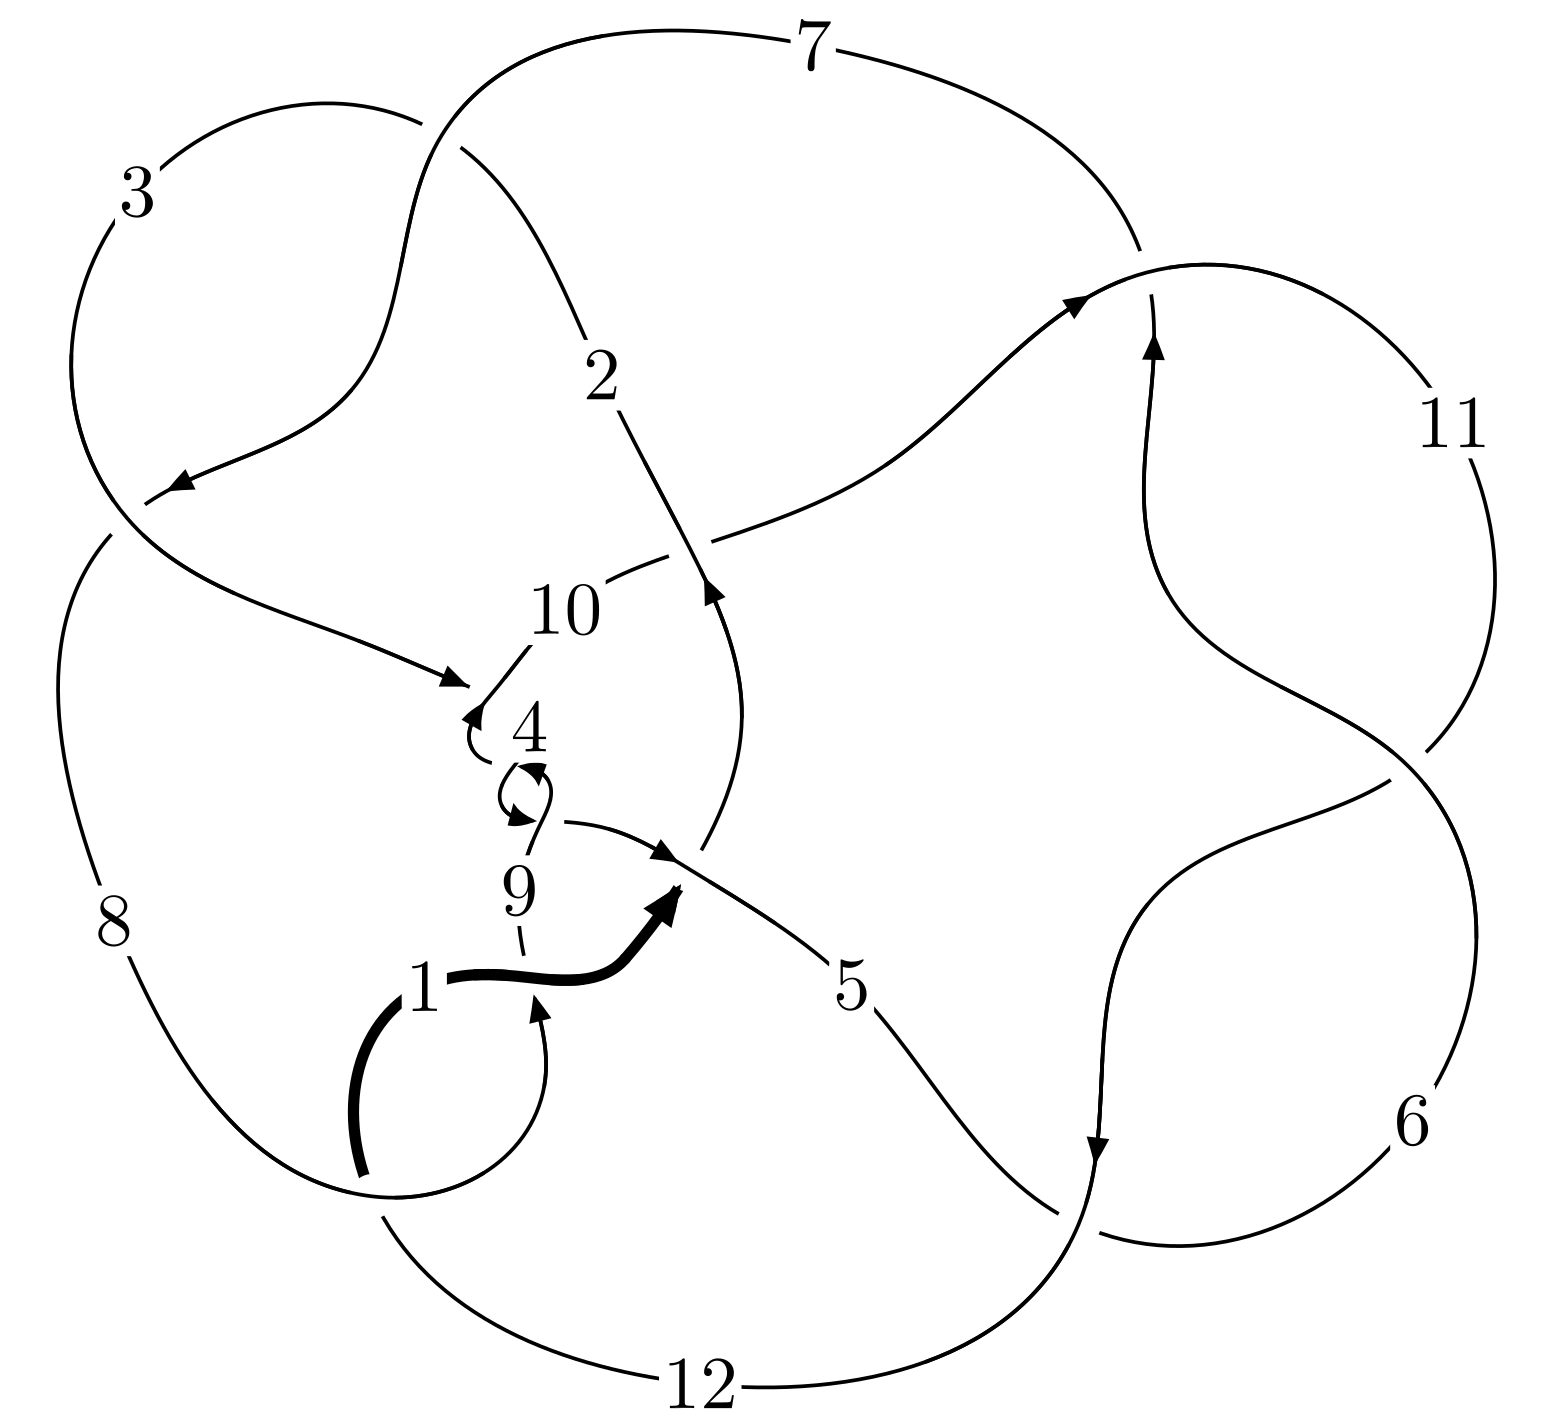
\includegraphics[width=112pt]{../../../GIT/diagram.site/Diagrams/png/2068_12a_1267.png}\\
\ \ \ A knot diagram\footnotemark}&
\allowdisplaybreaks
\textbf{Linearized knot diagam} \\
\cline{2-2}
 &
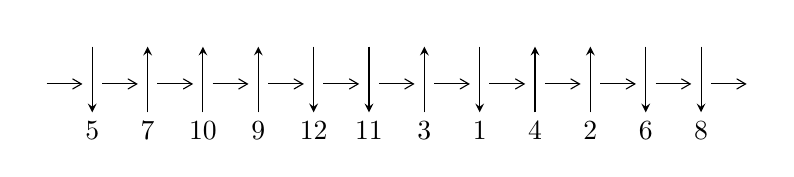
\begin{tikzpicture}[x=20pt, y=17pt]
	% nodes
	\node (C0) at (0, 0) {};
	\node (C1) at (1, 0) {};
	\node (C1U) at (1, +1) {};
	\node (C1D) at (1, -1) {5};

	\node (C2) at (2, 0) {};
	\node (C2U) at (2, +1) {};
	\node (C2D) at (2, -1) {7};

	\node (C3) at (3, 0) {};
	\node (C3U) at (3, +1) {};
	\node (C3D) at (3, -1) {10};

	\node (C4) at (4, 0) {};
	\node (C4U) at (4, +1) {};
	\node (C4D) at (4, -1) {9};

	\node (C5) at (5, 0) {};
	\node (C5U) at (5, +1) {};
	\node (C5D) at (5, -1) {12};

	\node (C6) at (6, 0) {};
	\node (C6U) at (6, +1) {};
	\node (C6D) at (6, -1) {11};

	\node (C7) at (7, 0) {};
	\node (C7U) at (7, +1) {};
	\node (C7D) at (7, -1) {3};

	\node (C8) at (8, 0) {};
	\node (C8U) at (8, +1) {};
	\node (C8D) at (8, -1) {1};

	\node (C9) at (9, 0) {};
	\node (C9U) at (9, +1) {};
	\node (C9D) at (9, -1) {4};

	\node (C10) at (10, 0) {};
	\node (C10U) at (10, +1) {};
	\node (C10D) at (10, -1) {2};

	\node (C11) at (11, 0) {};
	\node (C11U) at (11, +1) {};
	\node (C11D) at (11, -1) {6};

	\node (C12) at (12, 0) {};
	\node (C12U) at (12, +1) {};
	\node (C12D) at (12, -1) {8};
	\node (C13) at (13, 0) {};

	% arrows
	\draw[->,>={angle 60}]
	(C0) edge (C1) (C1) edge (C2) (C2) edge (C3) (C3) edge (C4) (C4) edge (C5) (C5) edge (C6) (C6) edge (C7) (C7) edge (C8) (C8) edge (C9) (C9) edge (C10) (C10) edge (C11) (C11) edge (C12) (C12) edge (C13) ;	\draw[->,>=stealth]
	(C1U) edge (C1D) (C2D) edge (C2U) (C3D) edge (C3U) (C4D) edge (C4U) (C5U) edge (C5D) (C6U) edge (C6D) (C7D) edge (C7U) (C8U) edge (C8D) (C9D) edge (C9U) (C10D) edge (C10U) (C11U) edge (C11D) (C12U) edge (C12D) ;
	\end{tikzpicture} \\
\hhline{~~} \\& 
\textbf{Solving Sequence} \\ \cline{2-2} 
 &
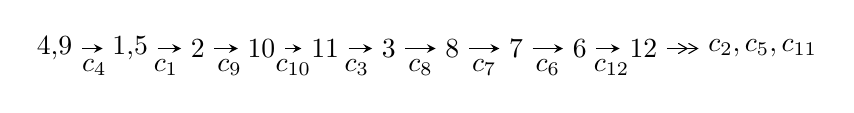
\begin{tikzpicture}[x=23pt, y=7pt]
	% node
	\node (A0) at (-1/8, 0) {4,9};
	\node (A1) at (17/16, 0) {1,5};
	\node (A2) at (17/8, 0) {2};
	\node (A3) at (25/8, 0) {10};
	\node (A4) at (33/8, 0) {11};
	\node (A5) at (41/8, 0) {3};
	\node (A6) at (49/8, 0) {8};
	\node (A7) at (57/8, 0) {7};
	\node (A8) at (65/8, 0) {6};
	\node (A9) at (73/8, 0) {12};
	\node (C1) at (1/2, -1) {$c_{4}$};
	\node (C2) at (13/8, -1) {$c_{1}$};
	\node (C3) at (21/8, -1) {$c_{9}$};
	\node (C4) at (29/8, -1) {$c_{10}$};
	\node (C5) at (37/8, -1) {$c_{3}$};
	\node (C6) at (45/8, -1) {$c_{8}$};
	\node (C7) at (53/8, -1) {$c_{7}$};
	\node (C8) at (61/8, -1) {$c_{6}$};
	\node (C9) at (69/8, -1) {$c_{12}$};
	\node (A10) at (11, 0) {$c_{2},c_{5},c_{11}$};

	% edge
	\draw[->,>=stealth]	
	(A0) edge (A1) (A1) edge (A2) (A2) edge (A3) (A3) edge (A4) (A4) edge (A5) (A5) edge (A6) (A6) edge (A7) (A7) edge (A8) (A8) edge (A9) ;
	\draw[->>,>={angle 60}]	
	(A9) edge (A10);
\end{tikzpicture} \\ 

\end{tabular} \\

\footnotetext{
The image of knot diagram is generated by the software ``\textbf{Draw programme}" developed by Andrew Bartholomew(\url{http://www.layer8.co.uk/maths/draw/index.htm\#Running-draw}), where we modified some parts for our purpose(\url{https://github.com/CATsTAILs/LinksPainter}).
}\phantom \\ \newline 
\centering \textbf{Ideals for irreducible components\footnotemark of $X_{\text{par}}$} 
 
\begin{align*}
I^u_{1}&=\langle 
8.25299\times10^{186} u^{85}-5.27253\times10^{186} u^{84}+\cdots+1.79012\times10^{186} b+8.66584\times10^{186},\\
\phantom{I^u_{1}}&\phantom{= \langle  }-1.26969\times10^{188} u^{85}+1.78691\times10^{188} u^{84}+\cdots+1.25308\times10^{187} a-1.51944\times10^{188},\\
\phantom{I^u_{1}}&\phantom{= \langle  }3 u^{86}-3 u^{85}+\cdots+4 u+1\rangle \\
I^u_{2}&=\langle 
18 u^{13}-174 u^{12}+\cdots+89 b-27,\;75 u^{13}-102 u^{12}+\cdots+89 a-157,\\
\phantom{I^u_{2}}&\phantom{= \langle  }3 u^{14}+26 u^{12}+88 u^{10}- u^9+145 u^8-5 u^7+117 u^6-8 u^5+40 u^4-4 u^3+5 u^2+1\rangle \\
\\
\end{align*}
\raggedright * 2 irreducible components of $\dim_{\mathbb{C}}=0$, with total 100 representations.\\
\footnotetext{All coefficients of polynomials are rational numbers. But the coefficients are sometimes approximated in decimal forms when there is not enough margin.}
\newpage
\renewcommand{\arraystretch}{1}
\centering \section*{I. $I^u_{1}= \langle 8.25\times10^{186} u^{85}-5.27\times10^{186} u^{84}+\cdots+1.79\times10^{186} b+8.67\times10^{186},\;-1.27\times10^{188} u^{85}+1.79\times10^{188} u^{84}+\cdots+1.25\times10^{187} a-1.52\times10^{188},\;3 u^{86}-3 u^{85}+\cdots+4 u+1 \rangle$}
\flushleft \textbf{(i) Arc colorings}\\
\begin{tabular}{m{7pt} m{180pt} m{7pt} m{180pt} }
\flushright $a_{4}=$&$\begin{pmatrix}1\\0\end{pmatrix}$ \\
\flushright $a_{9}=$&$\begin{pmatrix}0\\u\end{pmatrix}$ \\
\flushright $a_{1}=$&$\begin{pmatrix}10.1325 u^{85}-14.2601 u^{84}+\cdots+33.2708 u+12.1256\\-4.61031 u^{85}+2.94535 u^{84}+\cdots-0.310845 u-4.84093\end{pmatrix}$ \\
\flushright $a_{5}=$&$\begin{pmatrix}1\\- u^2\end{pmatrix}$ \\
\flushright $a_{2}=$&$\begin{pmatrix}12.8237 u^{85}-16.0117 u^{84}+\cdots+31.4557 u+15.5907\\-3.45859 u^{85}+4.30170 u^{84}+\cdots+1.83913 u-4.52771\end{pmatrix}$ \\
\flushright $a_{10}=$&$\begin{pmatrix}u\\u\end{pmatrix}$ \\
\flushright $a_{11}=$&$\begin{pmatrix}-1.12037 u^{85}+0.720337 u^{84}+\cdots+17.0454 u+0.878741\\-2.47836 u^{85}+1.02170 u^{84}+\cdots+4.70916 u-6.99628\end{pmatrix}$ \\
\flushright $a_{3}=$&$\begin{pmatrix}u^2+1\\u^2\end{pmatrix}$ \\
\flushright $a_{8}=$&$\begin{pmatrix}-17.5488 u^{85}+22.2190 u^{84}+\cdots+16.4041 u-18.0315\\-4.97010 u^{85}+7.09366 u^{84}+\cdots-1.24274 u-5.11704\end{pmatrix}$ \\
\flushright $a_{7}=$&$\begin{pmatrix}-14.4489 u^{85}+18.7957 u^{84}+\cdots+18.7718 u-13.3281\\-6.11026 u^{85}+9.21618 u^{84}+\cdots-0.915132 u-4.68180\end{pmatrix}$ \\
\flushright $a_{6}=$&$\begin{pmatrix}-14.2020 u^{85}+17.7124 u^{84}+\cdots-7.96939 u-10.9258\\0.953032 u^{85}-2.63390 u^{84}+\cdots+7.75357 u+2.84298\end{pmatrix}$ \\
\flushright $a_{12}=$&$\begin{pmatrix}-0.365418 u^{85}+0.299031 u^{84}+\cdots-12.0524 u-1.61229\\-3.84456 u^{85}+3.13245 u^{84}+\cdots-0.840605 u-6.14246\end{pmatrix}$\\&\end{tabular}
\flushleft \textbf{(ii) Obstruction class $= -1$}\\~\\
\flushleft \textbf{(iii) Cusp Shapes $= 8.37795 u^{85}-7.06948 u^{84}+\cdots-60.2641 u+24.3494$}\\~\\
\newpage\renewcommand{\arraystretch}{1}
\flushleft \textbf{(iv) u-Polynomials at the component}\newline \\
\begin{tabular}{m{50pt}|m{274pt}}
Crossings & \hspace{64pt}u-Polynomials at each crossing \\
\hline $$\begin{aligned}c_{1}\end{aligned}$$&$\begin{aligned}
&u^{86}+7 u^{85}+\cdots+486114 u+316869
\end{aligned}$\\
\hline $$\begin{aligned}c_{2},c_{7}\end{aligned}$$&$\begin{aligned}
&u^{86}+3 u^{85}+\cdots+148 u+799
\end{aligned}$\\
\hline $$\begin{aligned}c_{3},c_{4},c_{9}\end{aligned}$$&$\begin{aligned}
&3(3 u^{86}+3 u^{85}+\cdots-4 u+1)
\end{aligned}$\\
\hline $$\begin{aligned}c_{5},c_{6},c_{11}\end{aligned}$$&$\begin{aligned}
&3(3 u^{86}-3 u^{85}+\cdots+4 u+1)
\end{aligned}$\\
\hline $$\begin{aligned}c_{8},c_{12}\end{aligned}$$&$\begin{aligned}
&u^{86}-3 u^{85}+\cdots-148 u+799
\end{aligned}$\\
\hline $$\begin{aligned}c_{10}\end{aligned}$$&$\begin{aligned}
&u^{86}-7 u^{85}+\cdots-486114 u+316869
\end{aligned}$\\
\hline
\end{tabular}\\~\\
\newpage\renewcommand{\arraystretch}{1}
\flushleft \textbf{(v) Riley Polynomials at the component}\newline \\
\begin{tabular}{m{50pt}|m{274pt}}
Crossings & \hspace{64pt}Riley Polynomials at each crossing \\
\hline $$\begin{aligned}c_{1},c_{10}\end{aligned}$$&$\begin{aligned}
&y^{86}-21 y^{85}+\cdots-1166956777638 y+100405963161
\end{aligned}$\\
\hline $$\begin{aligned}c_{2},c_{7},c_{8}\\c_{12}\end{aligned}$$&$\begin{aligned}
&y^{86}-57 y^{85}+\cdots-19180326 y+638401
\end{aligned}$\\
\hline $$\begin{aligned}c_{3},c_{4},c_{5}\\c_{6},c_{9},c_{11}\end{aligned}$$&$\begin{aligned}
&9(9 y^{86}+873 y^{85}+\cdots-66 y+1)
\end{aligned}$\\
\hline
\end{tabular}\\~\\
\newpage\flushleft \textbf{(vi) Complex Volumes and Cusp Shapes}
$$\begin{array}{c|c|c}  
\text{Solutions to }I^u_{1}& \I (\text{vol} + \sqrt{-1}CS) & \text{Cusp shape}\\
 \hline 
\begin{aligned}
u &= -0.487671 + 0.911543 I \\
a &= -0.520086 - 0.799977 I \\
b &= -0.439016 - 1.321780 I\end{aligned}
 & -1.064110 + 0.470205 I & \phantom{-0.000000 } 0 \\ \hline\begin{aligned}
u &= -0.487671 - 0.911543 I \\
a &= -0.520086 + 0.799977 I \\
b &= -0.439016 + 1.321780 I\end{aligned}
 & -1.064110 - 0.470205 I & \phantom{-0.000000 } 0 \\ \hline\begin{aligned}
u &= \phantom{-}0.856002 + 0.610688 I \\
a &= \phantom{-}0.628665 - 1.135580 I \\
b &= -0.261332 - 1.147530 I\end{aligned}
 & \phantom{-}7.12197 + 12.14790 I & \phantom{-0.000000 } 0 \\ \hline\begin{aligned}
u &= \phantom{-}0.856002 - 0.610688 I \\
a &= \phantom{-}0.628665 + 1.135580 I \\
b &= -0.261332 + 1.147530 I\end{aligned}
 & \phantom{-}7.12197 - 12.14790 I & \phantom{-0.000000 } 0 \\ \hline\begin{aligned}
u &= \phantom{-}0.963439 + 0.540998 I \\
a &= -1.023910 + 0.143235 I \\
b &= \phantom{-}0.096072 + 0.494800 I\end{aligned}
 & \phantom{-}7.39198 - 6.24203 I & \phantom{-0.000000 } 0 \\ \hline\begin{aligned}
u &= \phantom{-}0.963439 - 0.540998 I \\
a &= -1.023910 - 0.143235 I \\
b &= \phantom{-}0.096072 - 0.494800 I\end{aligned}
 & \phantom{-}7.39198 + 6.24203 I & \phantom{-0.000000 } 0 \\ \hline\begin{aligned}
u &= -0.921313 + 0.623699 I \\
a &= \phantom{-}0.669038 + 0.884005 I \\
b &= -0.402135 + 1.000600 I\end{aligned}
 & \phantom{-0.000000 } -7.67590 I & \phantom{-0.000000 } 0 \\ \hline\begin{aligned}
u &= -0.921313 - 0.623699 I \\
a &= \phantom{-}0.669038 - 0.884005 I \\
b &= -0.402135 - 1.000600 I\end{aligned}
 & \phantom{-0.000000 -}7.67590 I & \phantom{-0.000000 } 0 \\ \hline\begin{aligned}
u &= \phantom{-}0.321220 + 0.803749 I \\
a &= \phantom{-}0.37667 + 1.46824 I \\
b &= -0.341366 + 0.788072 I\end{aligned}
 & \phantom{-}4.70459 + 3.23509 I & \phantom{-0.000000 } 0 \\ \hline\begin{aligned}
u &= \phantom{-}0.321220 - 0.803749 I \\
a &= \phantom{-}0.37667 - 1.46824 I \\
b &= -0.341366 - 0.788072 I\end{aligned}
 & \phantom{-}4.70459 - 3.23509 I & \phantom{-0.000000 } 0\\
 \hline 
 \end{array}$$\newpage$$\begin{array}{c|c|c}  
\text{Solutions to }I^u_{1}& \I (\text{vol} + \sqrt{-1}CS) & \text{Cusp shape}\\
 \hline 
\begin{aligned}
u &= -0.505194 + 0.690435 I \\
a &= -0.215663 + 0.821217 I \\
b &= -0.83631 + 1.34916 I\end{aligned}
 & \phantom{-}9.33013 + 2.31543 I & \phantom{-0.000000 } 0 \\ \hline\begin{aligned}
u &= -0.505194 - 0.690435 I \\
a &= -0.215663 - 0.821217 I \\
b &= -0.83631 - 1.34916 I\end{aligned}
 & \phantom{-}9.33013 - 2.31543 I & \phantom{-0.000000 } 0 \\ \hline\begin{aligned}
u &= \phantom{-}0.431731 + 1.091580 I \\
a &= -0.014101 - 0.384619 I \\
b &= -0.607306 - 0.957724 I\end{aligned}
 & \phantom{-}1.064110 + 0.470205 I & \phantom{-0.000000 } 0 \\ \hline\begin{aligned}
u &= \phantom{-}0.431731 - 1.091580 I \\
a &= -0.014101 + 0.384619 I \\
b &= -0.607306 + 0.957724 I\end{aligned}
 & \phantom{-}1.064110 - 0.470205 I & \phantom{-0.000000 } 0 \\ \hline\begin{aligned}
u &= \phantom{-}0.560237 + 0.564254 I \\
a &= -0.77532 + 1.23875 I \\
b &= -0.291815 + 1.153590 I\end{aligned}
 & -3.23212 + 3.41317 I & \phantom{-0.000000 } 0 \\ \hline\begin{aligned}
u &= \phantom{-}0.560237 - 0.564254 I \\
a &= -0.77532 - 1.23875 I \\
b &= -0.291815 - 1.153590 I\end{aligned}
 & -3.23212 - 3.41317 I & \phantom{-0.000000 } 0 \\ \hline\begin{aligned}
u &= -0.000759 + 1.241220 I \\
a &= \phantom{-}0.557676 + 0.663407 I \\
b &= -0.981779 + 0.464477 I\end{aligned}
 & \phantom{-}4.73562 + 2.64695 I & \phantom{-0.000000 } 0 \\ \hline\begin{aligned}
u &= -0.000759 - 1.241220 I \\
a &= \phantom{-}0.557676 - 0.663407 I \\
b &= -0.981779 - 0.464477 I\end{aligned}
 & \phantom{-}4.73562 - 2.64695 I & \phantom{-0.000000 } 0 \\ \hline\begin{aligned}
u &= -0.627267 + 0.407754 I \\
a &= -1.11760 + 0.99125 I \\
b &= \phantom{-}0.262891 + 0.167185 I\end{aligned}
 & \phantom{-}10.13040 - 6.27484 I & \phantom{-}6.40999 + 5.74696 I \\ \hline\begin{aligned}
u &= -0.627267 - 0.407754 I \\
a &= -1.11760 - 0.99125 I \\
b &= \phantom{-}0.262891 - 0.167185 I\end{aligned}
 & \phantom{-}10.13040 + 6.27484 I & \phantom{-}6.40999 - 5.74696 I\\
 \hline 
 \end{array}$$\newpage$$\begin{array}{c|c|c}  
\text{Solutions to }I^u_{1}& \I (\text{vol} + \sqrt{-1}CS) & \text{Cusp shape}\\
 \hline 
\begin{aligned}
u &= \phantom{-}0.726981 + 0.084860 I \\
a &= \phantom{-}1.41693 + 0.38257 I \\
b &= \phantom{-}0.767837 + 0.216395 I\end{aligned}
 & \phantom{-}7.23134 + 0.42251 I & \phantom{-}5.49191 + 0. I\phantom{ +0.000000I} \\ \hline\begin{aligned}
u &= \phantom{-}0.726981 - 0.084860 I \\
a &= \phantom{-}1.41693 - 0.38257 I \\
b &= \phantom{-}0.767837 - 0.216395 I\end{aligned}
 & \phantom{-}7.23134 - 0.42251 I & \phantom{-}5.49191 + 0. I\phantom{ +0.000000I} \\ \hline\begin{aligned}
u &= -0.596524 + 0.422138 I \\
a &= -1.02316 - 1.47258 I \\
b &= -0.315235 - 1.281800 I\end{aligned}
 & \phantom{-}2.30383 - 6.26437 I & \phantom{-}1.63409 + 7.43655 I \\ \hline\begin{aligned}
u &= -0.596524 - 0.422138 I \\
a &= -1.02316 + 1.47258 I \\
b &= -0.315235 + 1.281800 I\end{aligned}
 & \phantom{-}2.30383 + 6.26437 I & \phantom{-}1.63409 - 7.43655 I \\ \hline\begin{aligned}
u &= \phantom{-}0.287124 + 1.241250 I \\
a &= -0.244566 + 0.741804 I \\
b &= -0.909415 + 0.192812 I\end{aligned}
 & \phantom{-}3.16071 + 4.12903 I & \phantom{-0.000000 } 0 \\ \hline\begin{aligned}
u &= \phantom{-}0.287124 - 1.241250 I \\
a &= -0.244566 - 0.741804 I \\
b &= -0.909415 - 0.192812 I\end{aligned}
 & \phantom{-}3.16071 - 4.12903 I & \phantom{-0.000000 } 0 \\ \hline\begin{aligned}
u &= -0.235693 + 1.263220 I \\
a &= \phantom{-}0.032254 - 0.400412 I \\
b &= -0.555856 - 0.007715 I\end{aligned}
 & -1.86105 - 3.25299 I & \phantom{-0.000000 } 0 \\ \hline\begin{aligned}
u &= -0.235693 - 1.263220 I \\
a &= \phantom{-}0.032254 + 0.400412 I \\
b &= -0.555856 + 0.007715 I\end{aligned}
 & -1.86105 + 3.25299 I & \phantom{-0.000000 } 0 \\ \hline\begin{aligned}
u &= \phantom{-}0.631478 + 0.271047 I \\
a &= -0.591175 - 1.013090 I \\
b &= \phantom{-}0.344397 - 0.092151 I\end{aligned}
 & \phantom{-}3.23212 + 3.41317 I & \phantom{-}5.46052 - 6.79522 I \\ \hline\begin{aligned}
u &= \phantom{-}0.631478 - 0.271047 I \\
a &= -0.591175 + 1.013090 I \\
b &= \phantom{-}0.344397 + 0.092151 I\end{aligned}
 & \phantom{-}3.23212 - 3.41317 I & \phantom{-}5.46052 + 6.79522 I\\
 \hline 
 \end{array}$$\newpage$$\begin{array}{c|c|c}  
\text{Solutions to }I^u_{1}& \I (\text{vol} + \sqrt{-1}CS) & \text{Cusp shape}\\
 \hline 
\begin{aligned}
u &= -0.193356 + 0.653858 I \\
a &= \phantom{-}0.39714 - 1.66348 I \\
b &= -0.120691 - 0.722866 I\end{aligned}
 & -0.89196 - 2.61916 I & -5.06104 + 7.35063 I \\ \hline\begin{aligned}
u &= -0.193356 - 0.653858 I \\
a &= \phantom{-}0.39714 + 1.66348 I \\
b &= -0.120691 + 0.722866 I\end{aligned}
 & -0.89196 + 2.61916 I & -5.06104 - 7.35063 I \\ \hline\begin{aligned}
u &= -0.676515\phantom{ +0.000000I} \\
a &= \phantom{-}0.391689\phantom{ +0.000000I} \\
b &= \phantom{-}0.480875\phantom{ +0.000000I}\end{aligned}
 & \phantom{-}2.05833\phantom{ +0.000000I} & \phantom{-}4.89630\phantom{ +0.000000I} \\ \hline\begin{aligned}
u &= -0.673175\phantom{ +0.000000I} \\
a &= \phantom{-}0.969085\phantom{ +0.000000I} \\
b &= \phantom{-}0.605912\phantom{ +0.000000I}\end{aligned}
 & \phantom{-}1.99887\phantom{ +0.000000I} & \phantom{-}7.65390\phantom{ +0.000000I} \\ \hline\begin{aligned}
u &= -0.144636 + 1.328270 I \\
a &= \phantom{-}0.505549 - 0.495815 I \\
b &= -0.112467 - 0.581830 I\end{aligned}
 & -1.95971 - 2.93883 I & \phantom{-0.000000 } 0 \\ \hline\begin{aligned}
u &= -0.144636 - 1.328270 I \\
a &= \phantom{-}0.505549 + 0.495815 I \\
b &= -0.112467 + 0.581830 I\end{aligned}
 & -1.95971 + 2.93883 I & \phantom{-0.000000 } 0 \\ \hline\begin{aligned}
u &= \phantom{-}0.479835 + 0.420836 I \\
a &= \phantom{-}0.892610 + 1.003410 I \\
b &= \phantom{-}0.124839 + 0.664543 I\end{aligned}
 & \phantom{-}6.00993 + 1.65203 I & \phantom{-}4.77572 - 3.95144 I \\ \hline\begin{aligned}
u &= \phantom{-}0.479835 - 0.420836 I \\
a &= \phantom{-}0.892610 - 1.003410 I \\
b &= \phantom{-}0.124839 - 0.664543 I\end{aligned}
 & \phantom{-}6.00993 - 1.65203 I & \phantom{-}4.77572 + 3.95144 I \\ \hline\begin{aligned}
u &= -0.06042 + 1.41537 I \\
a &= -0.002140 + 0.690224 I \\
b &= -0.99592 + 4.19318 I\end{aligned}
 & \phantom{-}3.28875 - 4.65753 I & \phantom{-0.000000 } 0 \\ \hline\begin{aligned}
u &= -0.06042 - 1.41537 I \\
a &= -0.002140 - 0.690224 I \\
b &= -0.99592 - 4.19318 I\end{aligned}
 & \phantom{-}3.28875 + 4.65753 I & \phantom{-0.000000 } 0\\
 \hline 
 \end{array}$$\newpage$$\begin{array}{c|c|c}  
\text{Solutions to }I^u_{1}& \I (\text{vol} + \sqrt{-1}CS) & \text{Cusp shape}\\
 \hline 
\begin{aligned}
u &= -0.04706 + 1.42242 I \\
a &= \phantom{-}0.613070 - 1.016210 I \\
b &= \phantom{-}0.17258 - 2.46335 I\end{aligned}
 & -3.16071 - 4.12903 I & \phantom{-0.000000 } 0 \\ \hline\begin{aligned}
u &= -0.04706 - 1.42242 I \\
a &= \phantom{-}0.613070 + 1.016210 I \\
b &= \phantom{-}0.17258 + 2.46335 I\end{aligned}
 & -3.16071 + 4.12903 I & \phantom{-0.000000 } 0 \\ \hline\begin{aligned}
u &= \phantom{-}0.01657 + 1.43758 I \\
a &= \phantom{-}0.299100 + 1.063970 I \\
b &= -0.34288 + 2.97475 I\end{aligned}
 & -7.23134 + 0.42251 I & \phantom{-0.000000 } 0 \\ \hline\begin{aligned}
u &= \phantom{-}0.01657 - 1.43758 I \\
a &= \phantom{-}0.299100 - 1.063970 I \\
b &= -0.34288 - 2.97475 I\end{aligned}
 & -7.23134 - 0.42251 I & \phantom{-0.000000 } 0 \\ \hline\begin{aligned}
u &= \phantom{-}0.03499 + 1.44768 I \\
a &= \phantom{-}0.028434 - 0.897624 I \\
b &= -0.59814 - 3.42379 I\end{aligned}
 & -4.70459 + 3.23509 I & \phantom{-0.000000 } 0 \\ \hline\begin{aligned}
u &= \phantom{-}0.03499 - 1.44768 I \\
a &= \phantom{-}0.028434 + 0.897624 I \\
b &= -0.59814 + 3.42379 I\end{aligned}
 & -4.70459 - 3.23509 I & \phantom{-0.000000 } 0 \\ \hline\begin{aligned}
u &= \phantom{-}0.18665 + 1.43635 I \\
a &= \phantom{-}0.825892 + 0.184922 I \\
b &= \phantom{-}0.850357 + 0.231410 I\end{aligned}
 & -2.30383 + 6.26437 I & \phantom{-0.000000 } 0 \\ \hline\begin{aligned}
u &= \phantom{-}0.18665 - 1.43635 I \\
a &= \phantom{-}0.825892 - 0.184922 I \\
b &= \phantom{-}0.850357 - 0.231410 I\end{aligned}
 & -2.30383 - 6.26437 I & \phantom{-0.000000 } 0 \\ \hline\begin{aligned}
u &= \phantom{-}0.11480 + 1.44688 I \\
a &= -0.694209 - 0.053203 I \\
b &= -0.679675 - 0.653122 I\end{aligned}
 & \phantom{-0.000000 -}3.69188 I & \phantom{-0.000000 } 0 \\ \hline\begin{aligned}
u &= \phantom{-}0.11480 - 1.44688 I \\
a &= -0.694209 + 0.053203 I \\
b &= -0.679675 + 0.653122 I\end{aligned}
 & \phantom{-0.000000 } -3.69188 I & \phantom{-0.000000 } 0\\
 \hline 
 \end{array}$$\newpage$$\begin{array}{c|c|c}  
\text{Solutions to }I^u_{1}& \I (\text{vol} + \sqrt{-1}CS) & \text{Cusp shape}\\
 \hline 
\begin{aligned}
u &= -0.283866 + 0.467353 I \\
a &= \phantom{-}1.79360 + 1.70928 I \\
b &= \phantom{-}0.239555 + 0.361758 I\end{aligned}
 & \phantom{-}1.95971 + 2.93883 I & -0.481864 - 0.328566 I \\ \hline\begin{aligned}
u &= -0.283866 - 0.467353 I \\
a &= \phantom{-}1.79360 - 1.70928 I \\
b &= \phantom{-}0.239555 - 0.361758 I\end{aligned}
 & \phantom{-}1.95971 - 2.93883 I & -0.481864 + 0.328566 I \\ \hline\begin{aligned}
u &= -0.03514 + 1.45912 I \\
a &= -0.566579 + 0.046761 I \\
b &= -0.219530 + 0.313848 I\end{aligned}
 & -6.00993 - 1.65203 I & \phantom{-0.000000 } 0 \\ \hline\begin{aligned}
u &= -0.03514 - 1.45912 I \\
a &= -0.566579 - 0.046761 I \\
b &= -0.219530 - 0.313848 I\end{aligned}
 & -6.00993 + 1.65203 I & \phantom{-0.000000 } 0 \\ \hline\begin{aligned}
u &= -0.20070 + 1.48548 I \\
a &= \phantom{-}0.971535 + 0.007856 I \\
b &= \phantom{-}1.236640 + 0.079684 I\end{aligned}
 & \phantom{-}3.93602 - 9.24074 I & \phantom{-0.000000 } 0 \\ \hline\begin{aligned}
u &= -0.20070 - 1.48548 I \\
a &= \phantom{-}0.971535 - 0.007856 I \\
b &= \phantom{-}1.236640 - 0.079684 I\end{aligned}
 & \phantom{-}3.93602 + 9.24074 I & \phantom{-0.000000 } 0 \\ \hline\begin{aligned}
u &= -0.21298 + 1.48636 I \\
a &= -0.237402 + 0.916328 I \\
b &= \phantom{-}0.86614 + 3.02599 I\end{aligned}
 & -3.93602 - 9.24074 I & \phantom{-0.000000 } 0 \\ \hline\begin{aligned}
u &= -0.21298 - 1.48636 I \\
a &= -0.237402 - 0.916328 I \\
b &= \phantom{-}0.86614 - 3.02599 I\end{aligned}
 & -3.93602 + 9.24074 I & \phantom{-0.000000 } 0 \\ \hline\begin{aligned}
u &= \phantom{-}0.02339 + 1.52036 I \\
a &= -0.211488 - 1.106500 I \\
b &= -0.43560 - 3.21969 I\end{aligned}
 & -4.73562 + 2.64695 I & \phantom{-0.000000 } 0 \\ \hline\begin{aligned}
u &= \phantom{-}0.02339 - 1.52036 I \\
a &= -0.211488 + 1.106500 I \\
b &= -0.43560 + 3.21969 I\end{aligned}
 & -4.73562 - 2.64695 I & \phantom{-0.000000 } 0\\
 \hline 
 \end{array}$$\newpage$$\begin{array}{c|c|c}  
\text{Solutions to }I^u_{1}& \I (\text{vol} + \sqrt{-1}CS) & \text{Cusp shape}\\
 \hline 
\begin{aligned}
u &= \phantom{-}0.19979 + 1.53163 I \\
a &= -0.172954 - 0.869817 I \\
b &= \phantom{-}0.68014 - 2.86249 I\end{aligned}
 & -10.13040 + 6.27484 I & \phantom{-0.000000 } 0 \\ \hline\begin{aligned}
u &= \phantom{-}0.19979 - 1.53163 I \\
a &= -0.172954 + 0.869817 I \\
b &= \phantom{-}0.68014 + 2.86249 I\end{aligned}
 & -10.13040 - 6.27484 I & \phantom{-0.000000 } 0 \\ \hline\begin{aligned}
u &= -0.223952 + 0.387967 I \\
a &= \phantom{-}0.618142 - 0.502973 I \\
b &= -0.169088 - 0.351297 I\end{aligned}
 & \phantom{-0.000000 } -0.900974 I & \phantom{-0.000000 -}0. + 7.50554 I \\ \hline\begin{aligned}
u &= -0.223952 - 0.387967 I \\
a &= \phantom{-}0.618142 + 0.502973 I \\
b &= -0.169088 + 0.351297 I\end{aligned}
 & \phantom{-0.000000 -}0.900974 I & \phantom{-0.000000 } 0. - 7.50554 I \\ \hline\begin{aligned}
u &= \phantom{-}0.434522\phantom{ +0.000000I} \\
a &= \phantom{-}2.58762\phantom{ +0.000000I} \\
b &= \phantom{-}0.222757\phantom{ +0.000000I}\end{aligned}
 & -2.05833\phantom{ +0.000000I} & -4.89630\phantom{ +0.000000I} \\ \hline\begin{aligned}
u &= -0.07485 + 1.56466 I \\
a &= -0.441297 + 0.905738 I \\
b &= -0.35616 + 2.76608 I\end{aligned}
 & -8.34474 - 3.71137 I & \phantom{-0.000000 } 0 \\ \hline\begin{aligned}
u &= -0.07485 - 1.56466 I \\
a &= -0.441297 - 0.905738 I \\
b &= -0.35616 - 2.76608 I\end{aligned}
 & -8.34474 + 3.71137 I & \phantom{-0.000000 } 0 \\ \hline\begin{aligned}
u &= \phantom{-}0.08170 + 1.59085 I \\
a &= -0.648395 - 0.893946 I \\
b &= -0.65822 - 2.54758 I\end{aligned}
 & -3.28875 + 4.65753 I & \phantom{-0.000000 } 0 \\ \hline\begin{aligned}
u &= \phantom{-}0.08170 - 1.59085 I \\
a &= -0.648395 + 0.893946 I \\
b &= -0.65822 + 2.54758 I\end{aligned}
 & -3.28875 - 4.65753 I & \phantom{-0.000000 } 0 \\ \hline\begin{aligned}
u &= \phantom{-}0.29800 + 1.57396 I \\
a &= \phantom{-}0.246710 + 0.935520 I \\
b &= -0.15569 + 3.07448 I\end{aligned}
 & \phantom{-0.000000 -}16.4101 I & \phantom{-0.000000 } 0\\
 \hline 
 \end{array}$$\newpage$$\begin{array}{c|c|c}  
\text{Solutions to }I^u_{1}& \I (\text{vol} + \sqrt{-1}CS) & \text{Cusp shape}\\
 \hline 
\begin{aligned}
u &= \phantom{-}0.29800 - 1.57396 I \\
a &= \phantom{-}0.246710 - 0.935520 I \\
b &= -0.15569 - 3.07448 I\end{aligned}
 & \phantom{-0.000000 } -16.4101 I & \phantom{-0.000000 } 0 \\ \hline\begin{aligned}
u &= -0.30827 + 1.57408 I \\
a &= \phantom{-}0.140960 - 0.917038 I \\
b &= -0.17590 - 3.00993 I\end{aligned}
 & -7.12197 - 12.14790 I & \phantom{-0.000000 } 0 \\ \hline\begin{aligned}
u &= -0.30827 - 1.57408 I \\
a &= \phantom{-}0.140960 + 0.917038 I \\
b &= -0.17590 + 3.00993 I\end{aligned}
 & -7.12197 + 12.14790 I & \phantom{-0.000000 } 0 \\ \hline\begin{aligned}
u &= -0.17904 + 1.60291 I \\
a &= -0.112096 + 0.747783 I \\
b &= \phantom{-}0.52909 + 2.60371 I\end{aligned}
 & -9.33013 - 2.31543 I & \phantom{-0.000000 } 0 \\ \hline\begin{aligned}
u &= -0.17904 - 1.60291 I \\
a &= -0.112096 - 0.747783 I \\
b &= \phantom{-}0.52909 - 2.60371 I\end{aligned}
 & -9.33013 + 2.31543 I & \phantom{-0.000000 } 0 \\ \hline\begin{aligned}
u &= \phantom{-}0.34500 + 1.57965 I \\
a &= \phantom{-}0.006689 + 0.841214 I \\
b &= -0.15345 + 2.86415 I\end{aligned}
 & -7.39198 + 6.24203 I & \phantom{-0.000000 } 0 \\ \hline\begin{aligned}
u &= \phantom{-}0.34500 - 1.57965 I \\
a &= \phantom{-}0.006689 - 0.841214 I \\
b &= -0.15345 - 2.86415 I\end{aligned}
 & -7.39198 - 6.24203 I & \phantom{-0.000000 } 0 \\ \hline\begin{aligned}
u &= -0.282381 + 0.029712 I \\
a &= \phantom{-}4.00451 + 2.52429 I \\
b &= \phantom{-}0.421921 + 0.008830 I\end{aligned}
 & \phantom{-}1.86105 - 3.25299 I & \phantom{-}5.47082 - 3.29014 I \\ \hline\begin{aligned}
u &= -0.282381 - 0.029712 I \\
a &= \phantom{-}4.00451 - 2.52429 I \\
b &= \phantom{-}0.421921 - 0.008830 I\end{aligned}
 & \phantom{-}1.86105 + 3.25299 I & \phantom{-}5.47082 + 3.29014 I \\ \hline\begin{aligned}
u &= \phantom{-}0.150688 + 0.214643 I \\
a &= -0.98298 + 3.63099 I \\
b &= \phantom{-}0.681811 + 0.988825 I\end{aligned}
 & \phantom{-}0.89196 + 2.61916 I & \phantom{-}5.06104 - 7.35063 I\\
 \hline 
 \end{array}$$\newpage$$\begin{array}{c|c|c}  
\text{Solutions to }I^u_{1}& \I (\text{vol} + \sqrt{-1}CS) & \text{Cusp shape}\\
 \hline 
\begin{aligned}
u &= \phantom{-}0.150688 - 0.214643 I \\
a &= -0.98298 - 3.63099 I \\
b &= \phantom{-}0.681811 - 0.988825 I\end{aligned}
 & \phantom{-}0.89196 - 2.61916 I & \phantom{-}5.06104 + 7.35063 I \\ \hline\begin{aligned}
u &= -0.229003 + 0.075392 I \\
a &= -2.35269 - 2.28645 I \\
b &= \phantom{-}1.19133 - 1.76013 I\end{aligned}
 & \phantom{-}8.34474 - 3.71137 I & \phantom{-}7.0250 + 12.9569 I \\ \hline\begin{aligned}
u &= -0.229003 - 0.075392 I \\
a &= -2.35269 + 2.28645 I \\
b &= \phantom{-}1.19133 + 1.76013 I\end{aligned}
 & \phantom{-}8.34474 + 3.71137 I & \phantom{-}7.0250 - 12.9569 I \\ \hline\begin{aligned}
u &= \phantom{-}0.161155\phantom{ +0.000000I} \\
a &= \phantom{-}7.85670\phantom{ +0.000000I} \\
b &= \phantom{-}0.573794\phantom{ +0.000000I}\end{aligned}
 & -1.99887\phantom{ +0.000000I} & -7.65390\phantom{ +0.000000I} \\ \hline\begin{aligned}
u &= \phantom{-}0.01745 + 2.15189 I \\
a &= \phantom{-}0.020095 - 0.458120 I \\
b &= \phantom{-}0.20772 - 2.77676 I\end{aligned}
 & \phantom{-0.000000 } -0.140881 I & \phantom{-0.000000 } 0 \\ \hline\begin{aligned}
u &= \phantom{-}0.01745 - 2.15189 I \\
a &= \phantom{-}0.020095 + 0.458120 I \\
b &= \phantom{-}0.20772 + 2.77676 I\end{aligned}
 & \phantom{-0.000000 -}0.140881 I & \phantom{-0.000000 } 0\\
 \hline 
 \end{array}$$\newpage\newpage\renewcommand{\arraystretch}{1}
\centering \section*{II. $I^u_{2}= \langle 18 u^{13}-174 u^{12}+\cdots+89 b-27,\;75 u^{13}-102 u^{12}+\cdots+89 a-157,\;3 u^{14}+26 u^{12}+\cdots+5 u^2+1 \rangle$}
\flushleft \textbf{(i) Arc colorings}\\
\begin{tabular}{m{7pt} m{180pt} m{7pt} m{180pt} }
\flushright $a_{4}=$&$\begin{pmatrix}1\\0\end{pmatrix}$ \\
\flushright $a_{9}=$&$\begin{pmatrix}0\\u\end{pmatrix}$ \\
\flushright $a_{1}=$&$\begin{pmatrix}-0.842697 u^{13}+1.14607 u^{12}+\cdots-5.56180 u+1.76404\\-0.202247 u^{13}+1.95506 u^{12}+\cdots-2.13483 u+0.303371\end{pmatrix}$ \\
\flushright $a_{5}=$&$\begin{pmatrix}1\\- u^2\end{pmatrix}$ \\
\flushright $a_{2}=$&$\begin{pmatrix}0.438202 u^{13}-0.235955 u^{12}+\cdots-3.70787 u+1.84270\\0.438202 u^{13}-0.235955 u^{12}+\cdots-1.70787 u-0.157303\end{pmatrix}$ \\
\flushright $a_{10}=$&$\begin{pmatrix}u\\u\end{pmatrix}$ \\
\flushright $a_{11}=$&$\begin{pmatrix}3.84270 u^{13}+1.85393 u^{12}+\cdots-2.43820 u+2.23596\\0.842697 u^{13}+1.85393 u^{12}+\cdots+2.56180 u+1.23596\end{pmatrix}$ \\
\flushright $a_{3}=$&$\begin{pmatrix}u^2+1\\u^2\end{pmatrix}$ \\
\flushright $a_{8}=$&$\begin{pmatrix}-0.471910 u^{13}-0.438202 u^{12}+\cdots-7.31461 u+2.70787\\-0.235955 u^{13}-1.71910 u^{12}+\cdots-1.15730 u-0.146067\end{pmatrix}$ \\
\flushright $a_{7}=$&$\begin{pmatrix}-1.04494 u^{13}+0.101124 u^{12}+\cdots-6.69663 u+2.06742\\-2.66292 u^{13}-2.25843 u^{12}+\cdots-1.77528 u-0.505618\end{pmatrix}$ \\
\flushright $a_{6}=$&$\begin{pmatrix}-1.75281 u^{13}+0.943820 u^{12}+\cdots-13.1685 u+1.62921\\1.55056 u^{13}-1.98876 u^{12}+\cdots+0.0337079 u-1.32584\end{pmatrix}$ \\
\flushright $a_{12}=$&$\begin{pmatrix}-4.41573 u^{13}-1.31461 u^{12}+\cdots+1.05618 u-3.87640\\0.370787 u^{13}-1.58427 u^{12}+\cdots-0.752809 u-1.05618\end{pmatrix}$\\&\end{tabular}
\flushleft \textbf{(ii) Obstruction class $= 1$}\\~\\
\flushleft \textbf{(iii) Cusp Shapes $= -\frac{375}{89} u^{13}+\frac{777}{89} u^{12}-\frac{2929}{89} u^{11}+\frac{4610}{89} u^{10}-\frac{8245}{89} u^9+\frac{8241}{89} u^8-\frac{9589}{89} u^7+\frac{1708}{89} u^6-\frac{2626}{89} u^5-\frac{7109}{89} u^4+\frac{2607}{89} u^3-\frac{4498}{89} u^2+\frac{1263}{89} u-\frac{461}{89}$}\\~\\
\newpage\renewcommand{\arraystretch}{1}
\flushleft \textbf{(iv) u-Polynomials at the component}\newline \\
\begin{tabular}{m{50pt}|m{274pt}}
Crossings & \hspace{64pt}u-Polynomials at each crossing \\
\hline $$\begin{aligned}c_{1}\end{aligned}$$&$\begin{aligned}
&u^{14}+3 u^{12}+\cdots-6 u+3
\end{aligned}$\\
\hline $$\begin{aligned}c_{2},c_{12}\end{aligned}$$&$\begin{aligned}
&u^{14}-2 u^{13}+\cdots-2 u+1
\end{aligned}$\\
\hline $$\begin{aligned}c_{3},c_{4},c_{11}\end{aligned}$$&$\begin{aligned}
&3(3 u^{14}+26 u^{12}+\cdots+5 u^2+1)
\end{aligned}$\\
\hline $$\begin{aligned}c_{5},c_{6},c_{9}\end{aligned}$$&$\begin{aligned}
&3(3 u^{14}+26 u^{12}+\cdots+5 u^2+1)
\end{aligned}$\\
\hline $$\begin{aligned}c_{7},c_{8}\end{aligned}$$&$\begin{aligned}
&u^{14}+2 u^{13}+\cdots+2 u+1
\end{aligned}$\\
\hline $$\begin{aligned}c_{10}\end{aligned}$$&$\begin{aligned}
&u^{14}+3 u^{12}+\cdots+6 u+3
\end{aligned}$\\
\hline
\end{tabular}\\~\\
\newpage\renewcommand{\arraystretch}{1}
\flushleft \textbf{(v) Riley Polynomials at the component}\newline \\
\begin{tabular}{m{50pt}|m{274pt}}
Crossings & \hspace{64pt}Riley Polynomials at each crossing \\
\hline $$\begin{aligned}c_{1},c_{10}\end{aligned}$$&$\begin{aligned}
&y^{14}+6 y^{13}+\cdots+138 y+9
\end{aligned}$\\
\hline $$\begin{aligned}c_{2},c_{7},c_{8}\\c_{12}\end{aligned}$$&$\begin{aligned}
&y^{14}-10 y^{13}+\cdots-10 y+1
\end{aligned}$\\
\hline $$\begin{aligned}c_{3},c_{4},c_{5}\\c_{6},c_{9},c_{11}\end{aligned}$$&$\begin{aligned}
&9(9 y^{14}+156 y^{13}+\cdots+10 y+1)
\end{aligned}$\\
\hline
\end{tabular}\\~\\
\newpage\flushleft \textbf{(vi) Complex Volumes and Cusp Shapes}
$$\begin{array}{c|c|c}  
\text{Solutions to }I^u_{2}& \I (\text{vol} + \sqrt{-1}CS) & \text{Cusp shape}\\
 \hline 
\begin{aligned}
u &= -0.049553 + 0.816998 I \\
a &= \phantom{-}0.622815 + 1.051080 I \\
b &= \phantom{-}0.255119 + 1.055430 I\end{aligned}
 & \phantom{-0.000000 -}1.85654 I & \phantom{-0.000000 } 0. - 2.13171 I \\ \hline\begin{aligned}
u &= -0.049553 - 0.816998 I \\
a &= \phantom{-}0.622815 - 1.051080 I \\
b &= \phantom{-}0.255119 - 1.055430 I\end{aligned}
 & \phantom{-0.000000 } -1.85654 I & \phantom{-0.000000 -}0. + 2.13171 I \\ \hline\begin{aligned}
u &= -0.166900 + 1.243020 I \\
a &= \phantom{-}0.200539 - 0.505880 I \\
b &= -0.307932 + 0.212975 I\end{aligned}
 & -1.67379 - 3.65413 I & \phantom{-}2.66692 + 12.62316 I \\ \hline\begin{aligned}
u &= -0.166900 - 1.243020 I \\
a &= \phantom{-}0.200539 + 0.505880 I \\
b &= -0.307932 - 0.212975 I\end{aligned}
 & -1.67379 + 3.65413 I & \phantom{-}2.66692 - 12.62316 I \\ \hline\begin{aligned}
u &= \phantom{-}0.119392 + 1.297390 I \\
a &= \phantom{-}0.206627 + 0.369905 I \\
b &= -0.61057 - 1.43823 I\end{aligned}
 & \phantom{-}4.75184 + 4.77157 I & \phantom{-}5.13799 - 5.06722 I \\ \hline\begin{aligned}
u &= \phantom{-}0.119392 - 1.297390 I \\
a &= \phantom{-}0.206627 - 0.369905 I \\
b &= -0.61057 + 1.43823 I\end{aligned}
 & \phantom{-}4.75184 - 4.77157 I & \phantom{-}5.13799 + 5.06722 I \\ \hline\begin{aligned}
u &= -0.07305 + 1.52385 I \\
a &= -0.623956 + 1.010240 I \\
b &= -0.56152 + 2.77414 I\end{aligned}
 & -4.75184 - 4.77157 I & -5.13799 + 5.06722 I \\ \hline\begin{aligned}
u &= -0.07305 - 1.52385 I \\
a &= -0.623956 - 1.010240 I \\
b &= -0.56152 - 2.77414 I\end{aligned}
 & -4.75184 + 4.77157 I & -5.13799 - 5.06722 I \\ \hline\begin{aligned}
u &= \phantom{-}0.313574 + 0.311781 I \\
a &= \phantom{-}1.44019 - 0.55383 I \\
b &= \phantom{-}0.64911 - 1.78138 I\end{aligned}
 & \phantom{-}8.19608 - 3.29147 I & \phantom{-}0.69516 - 3.25780 I \\ \hline\begin{aligned}
u &= \phantom{-}0.313574 - 0.311781 I \\
a &= \phantom{-}1.44019 + 0.55383 I \\
b &= \phantom{-}0.64911 + 1.78138 I\end{aligned}
 & \phantom{-}8.19608 + 3.29147 I & \phantom{-}0.69516 + 3.25780 I\\
 \hline 
 \end{array}$$\newpage$$\begin{array}{c|c|c}  
\text{Solutions to }I^u_{2}& \I (\text{vol} + \sqrt{-1}CS) & \text{Cusp shape}\\
 \hline 
\begin{aligned}
u &= \phantom{-}0.10498 + 1.57135 I \\
a &= -0.317975 - 0.874627 I \\
b &= -0.18321 - 2.77269 I\end{aligned}
 & -8.19608 + 3.29147 I & -0.69516 + 3.25780 I \\ \hline\begin{aligned}
u &= \phantom{-}0.10498 - 1.57135 I \\
a &= -0.317975 + 0.874627 I \\
b &= -0.18321 + 2.77269 I\end{aligned}
 & -8.19608 - 3.29147 I & -0.69516 - 3.25780 I \\ \hline\begin{aligned}
u &= -0.248446 + 0.321511 I \\
a &= -0.52824 - 3.56716 I \\
b &= -0.240997 - 0.492814 I\end{aligned}
 & \phantom{-}1.67379 - 3.65413 I & -2.66692 + 12.62316 I \\ \hline\begin{aligned}
u &= -0.248446 - 0.321511 I \\
a &= -0.52824 + 3.56716 I \\
b &= -0.240997 + 0.492814 I\end{aligned}
 & \phantom{-}1.67379 + 3.65413 I & -2.66692 - 12.62316 I\\
 \hline 
 \end{array}$$\newpage
\newpage\renewcommand{\arraystretch}{1}
\centering \section*{ III. u-Polynomials}
\begin{tabular}{m{50pt}|m{274pt}}
Crossings & \hspace{64pt}u-Polynomials at each crossing \\
\hline $$\begin{aligned}c_{1}\end{aligned}$$&$\begin{aligned}
&(u^{14}+3 u^{12}+\cdots-6 u+3)(u^{86}+7 u^{85}+\cdots+486114 u+316869)
\end{aligned}$\\
\hline $$\begin{aligned}c_{2}\end{aligned}$$&$\begin{aligned}
&(u^{14}-2 u^{13}+\cdots-2 u+1)(u^{86}+3 u^{85}+\cdots+148 u+799)
\end{aligned}$\\
\hline $$\begin{aligned}c_{3},c_{4}\end{aligned}$$&$\begin{aligned}
&9(3 u^{14}+26 u^{12}+\cdots+5 u^2+1)(3 u^{86}+3 u^{85}+\cdots-4 u+1)
\end{aligned}$\\
\hline $$\begin{aligned}c_{5},c_{6}\end{aligned}$$&$\begin{aligned}
&9(3 u^{14}+26 u^{12}+\cdots+5 u^2+1)(3 u^{86}-3 u^{85}+\cdots+4 u+1)
\end{aligned}$\\
\hline $$\begin{aligned}c_{7}\end{aligned}$$&$\begin{aligned}
&(u^{14}+2 u^{13}+\cdots+2 u+1)(u^{86}+3 u^{85}+\cdots+148 u+799)
\end{aligned}$\\
\hline $$\begin{aligned}c_{8}\end{aligned}$$&$\begin{aligned}
&(u^{14}+2 u^{13}+\cdots+2 u+1)(u^{86}-3 u^{85}+\cdots-148 u+799)
\end{aligned}$\\
\hline $$\begin{aligned}c_{9}\end{aligned}$$&$\begin{aligned}
&9(3 u^{14}+26 u^{12}+\cdots+5 u^2+1)(3 u^{86}+3 u^{85}+\cdots-4 u+1)
\end{aligned}$\\
\hline $$\begin{aligned}c_{10}\end{aligned}$$&$\begin{aligned}
&(u^{14}+3 u^{12}+\cdots+6 u+3)(u^{86}-7 u^{85}+\cdots-486114 u+316869)
\end{aligned}$\\
\hline $$\begin{aligned}c_{11}\end{aligned}$$&$\begin{aligned}
&9(3 u^{14}+26 u^{12}+\cdots+5 u^2+1)(3 u^{86}-3 u^{85}+\cdots+4 u+1)
\end{aligned}$\\
\hline $$\begin{aligned}c_{12}\end{aligned}$$&$\begin{aligned}
&(u^{14}-2 u^{13}+\cdots-2 u+1)(u^{86}-3 u^{85}+\cdots-148 u+799)
\end{aligned}$\\
\hline
\end{tabular}\newpage\renewcommand{\arraystretch}{1}
\centering \section*{ IV. Riley Polynomials}
\begin{tabular}{m{50pt}|m{274pt}}
Crossings & \hspace{64pt}Riley Polynomials at each crossing \\
\hline $$\begin{aligned}c_{1},c_{10}\end{aligned}$$&$\begin{aligned}
&(y^{14}+6 y^{13}+\cdots+138 y+9)\\
&\cdot(y^{86}-21 y^{85}+\cdots-1166956777638 y+100405963161)
\end{aligned}$\\
\hline $$\begin{aligned}c_{2},c_{7},c_{8}\\c_{12}\end{aligned}$$&$\begin{aligned}
&(y^{14}-10 y^{13}+\cdots-10 y+1)\\
&\cdot(y^{86}-57 y^{85}+\cdots-19180326 y+638401)
\end{aligned}$\\
\hline $$\begin{aligned}c_{3},c_{4},c_{5}\\c_{6},c_{9},c_{11}\end{aligned}$$&$\begin{aligned}
&81(9 y^{14}+156 y^{13}+\cdots+10 y+1)(9 y^{86}+873 y^{85}+\cdots-66 y+1)
\end{aligned}$\\
\hline
\end{tabular}
\vskip 2pc
\end{document}